\chapter{MÉTODO SÍSMICO DE REFLEXÃO}
\label{cap.2}

O método sísmico de reflexão, consiste, basicamente, em obter informações da subsuperfície através da propagação de ondas produzidas por fontes artificiais em superfície e o posterior registro dessas ondas em receptores (geofones), que estão em superfície.
As ondas geradas pelas fontes propagam-se na subsuperfície, sendo transmitidas, refletidas e difratadas por interfaces geológicas que delimitam as camadas de rochas de diferentes propriedades físicas.
As ondas registradas nos receptores são provenientes das reflexões das interfaces, o sinal registrado pelos receptores possuem informações sob as ondas propagadas e suas mudanças conforme o trajeto do percusso da onda.


O metódo sísmico baseia-se na propagação do campo de onda, ou seja, na evolução temporal e espacial da frente de onda através de um meio com propriedades distintas e específicas, nas quais afetam diretamente a energia síssmica em propagação, fazendo-se necessário o estudo da equação da onda para compreender os fenômenos físicos envolvidos.

O campo de onda propagado é representado através de raios, que são retas perpendiculares as frentes de ondas (esféricas) com origem na fonte sísmica (perturbação).

O que se deseja no experimento sísmico é estimativa do tempo de trânsito ($\tau$) ao longo de uma trajetória qualquer referente a pares fonte-receptor, este pode ser calculado baseada no traçamento de raios e na lei de Snell para cada interface atravessada. Neste cálculo é empregada a equação iconal (equação \ref{eq:iconal}). Esta equação depende do conhecimento da distribuição das velocidades intervalares do modelo.

\begin{equation}
(\nabla \tau)^{2}=\frac{1}{v^{2}}
\label{eq:iconal}
\end{equation}

\section{MODELAGEM DA ESTRUTURA GEOLÓGICA}

O objetivo da modelagem de uma seção sísmica é a construção de um modelo que represente a subsuperfície de forma coerente geologicamente. A modelagem sísmica pode ser feita de forma direta e inversa a primeira é realizada quando se parte de um modelo geológico ``a priori'' onde conhecendo os parâmetros (velocidade, densidade), é gerada a resposta da energia de amplitude das ondas propagadas sob a condição da geometria das interfaces e camadas, registradas no sismograma sintético. Já na modelagem inversa, tem-se a resposta sísmica da subsuperfície e a partir da resposta, tenta-se então estimar os parâmetros sísmicos para construir um modelo geológico conciso a essas propriedades estimadas.

A modelagem direta, ou seja, o processo através do qual um modelo geológico de subsuperfície, em uma, duas ou três dimensões, é transformado em um registro sísmico sintético de dimensão correspondente, foi primeiramente usado por exploracionistas na década de 50 \cite{Edwards(1988)}.

A modelagem sísmica consiste de um sistema de equações diferenciais parciais (geralmente equações da onda acústicas, elásticas, visco-elásticas, etc.) acompanhadas das condições de contorno (comportamento nas interfaces e bordas do modelo) e condições iniciais (caracterização da emissão de energia pela fonte, tempo de propagação requerido, etc.). Na modelagem acústica na ausência de fontes internas, o sistema de equações diferenciais que expressa a resposta de um modelo geológico a um campo de ondas incidente, é constituído de equações da onda do tipo:

\begin{equation}
\nabla^{2}P(\mathbf{x},t)-\frac{1}{v^{2}}\frac{\partial^{2}}{\partial t^{2}}P(\mathbf{x},t)= 0,
\label{eq:Equacao_onda_acustica_0}
\end{equation}


O pacote Seismic Unix (SU) oferece subrotinas de modelagem e processamento de dados sísmicos, pode-se dividir em três grandes etapas este relatório:

\begin{itemize}
\item Criação do modelo pela subrotina \textit{trimodel}.
\item Aquisição do modelo (simulação do experimento sísmico).
\end{itemize}

Para a modelagem da estrutura geológica foi usada a subrotina \textit{trimodel} do pacote SU, esta rotina se baseia na triangulação de Delaunay. Este método sofisticado de geração de gráficos e imagens digitais, em duas ou três dimensões, é amplamente utilizado para modelar
a superfície de objetos de diferentes complexidades. Foi desenvolvido em 1934 pelo matemático russo Boris Nikolaevich, e consiste em representar o objeto através de uma malha de triângulos que cumprem a condição de Delaunay: ``O interior da circunferência que circunscreve cada triângulo deve ser vazia'' \cite{Hale(1991)}.

\begin{figure}[H]
\centering
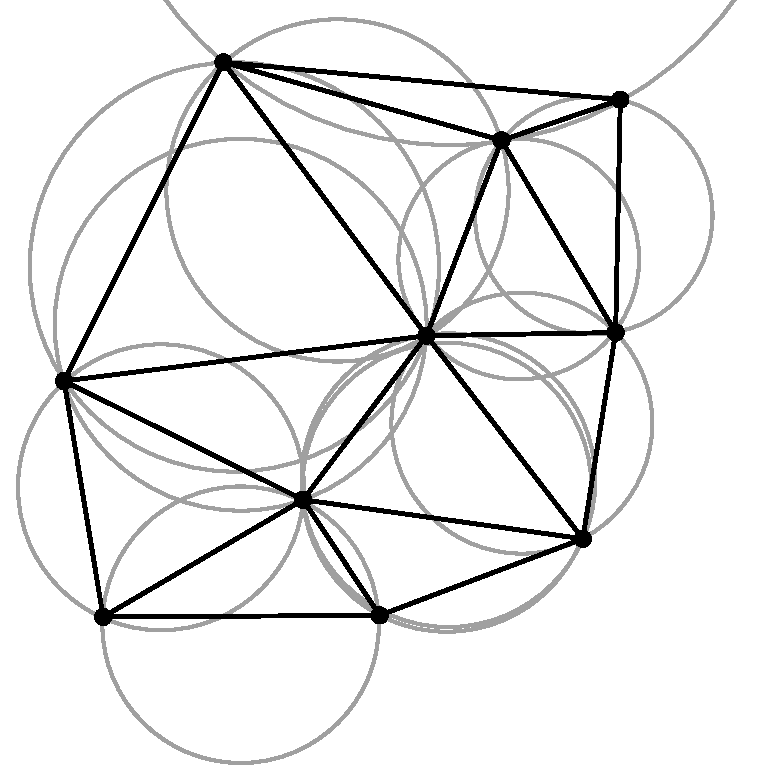
\includegraphics[width=7cm]{figuras/cap2/Delaunay_circumcircles_vectorial.pdf}
\caption{Triangulação de Delaunay no plano com as circunferências visíveis. Fonte: Wikipédia}
\label{fig:Delaunay_circumcircles_vectorial}
\end{figure}

A subrotina \textit{trimodel} do SU cria um modelo triangularizado, como mostra a figura (\ref{fig:vagarosidade}) a partir do modelo de velocidade da figura (\ref{fig:modelo_velocidade}). 
A velocidade é introduzida na forma de vagarosidade ($\textit{sloth}=1/v$), o método realiza o traçamento dos raios baseado na equação iconal \cite{Forel(2005)}. A vagarosidade ao quadrado das regiões (triângulos) é determinada pela equação (\ref{eq:vagarosidade}), onde o usuário define como é a variação da velocidade dentro de cada camada, na forma:

\begin{equation}
s(x,z)=s_{0}+\left(x-x_{0}\right) \frac{ds}{dx}+\left(z-z_{0}\right) \frac{ds}{dz}
\label{eq:vagarosidade}
\end{equation}

Cada par de x-z ainda é um ponto em uma camada. Na equação (\ref{eq:vagarosidade}) x, x0, z e z0 são os pontos finais e iniciais na horizontal e na vertical onde ocorrerá a variação da velocidade, esta variação terá um gradiente na direção x correspondente a $ds/dx$ e na direção z de magnitude $ds/dz$.

A descrição da subsuperfície requer uma representação matemática (modelagem numérica ou modelagem sísmica), as ondas sísmicas se propagação com diferentes velocidades em subsuperfície em função dos diferentes tipos de rochas em subsuperfície. A Tabela \ref{tab:tab1} apresenta os valores utilizados na construção do modelo de velocidade do modelo de camadas curvas (ver figura \ref{fig:modelo_velocidade}).

\begin{table}[H]
\centering
\begin{tabular}{|c|c|c|}
\hline
Camada & Velocidade da onda sísmica (m/s) & Vagarosidade $(m/s)^{-1}$ \\ \hline
1 & 1600 & 0.39 \\ \hline
2 & 1800 & 0.31 \\ \hline
3 & 1900 & 0.28 \\ \hline
4 & 2000 & 0.25 \\ \hline
5 & 1350 & 0.55 \\ \hline
6 & 1500 & 0.44 \\ \hline
7 & 2500 & 0.16 \\ \hline
\end{tabular}
\caption{Tabela de valores de vagarosidade e velocidade do modelo de camadas curvas.}
\label{tab:tab1}
\end{table}

\begin{landscape}
\begin{figure}[H]
\centering
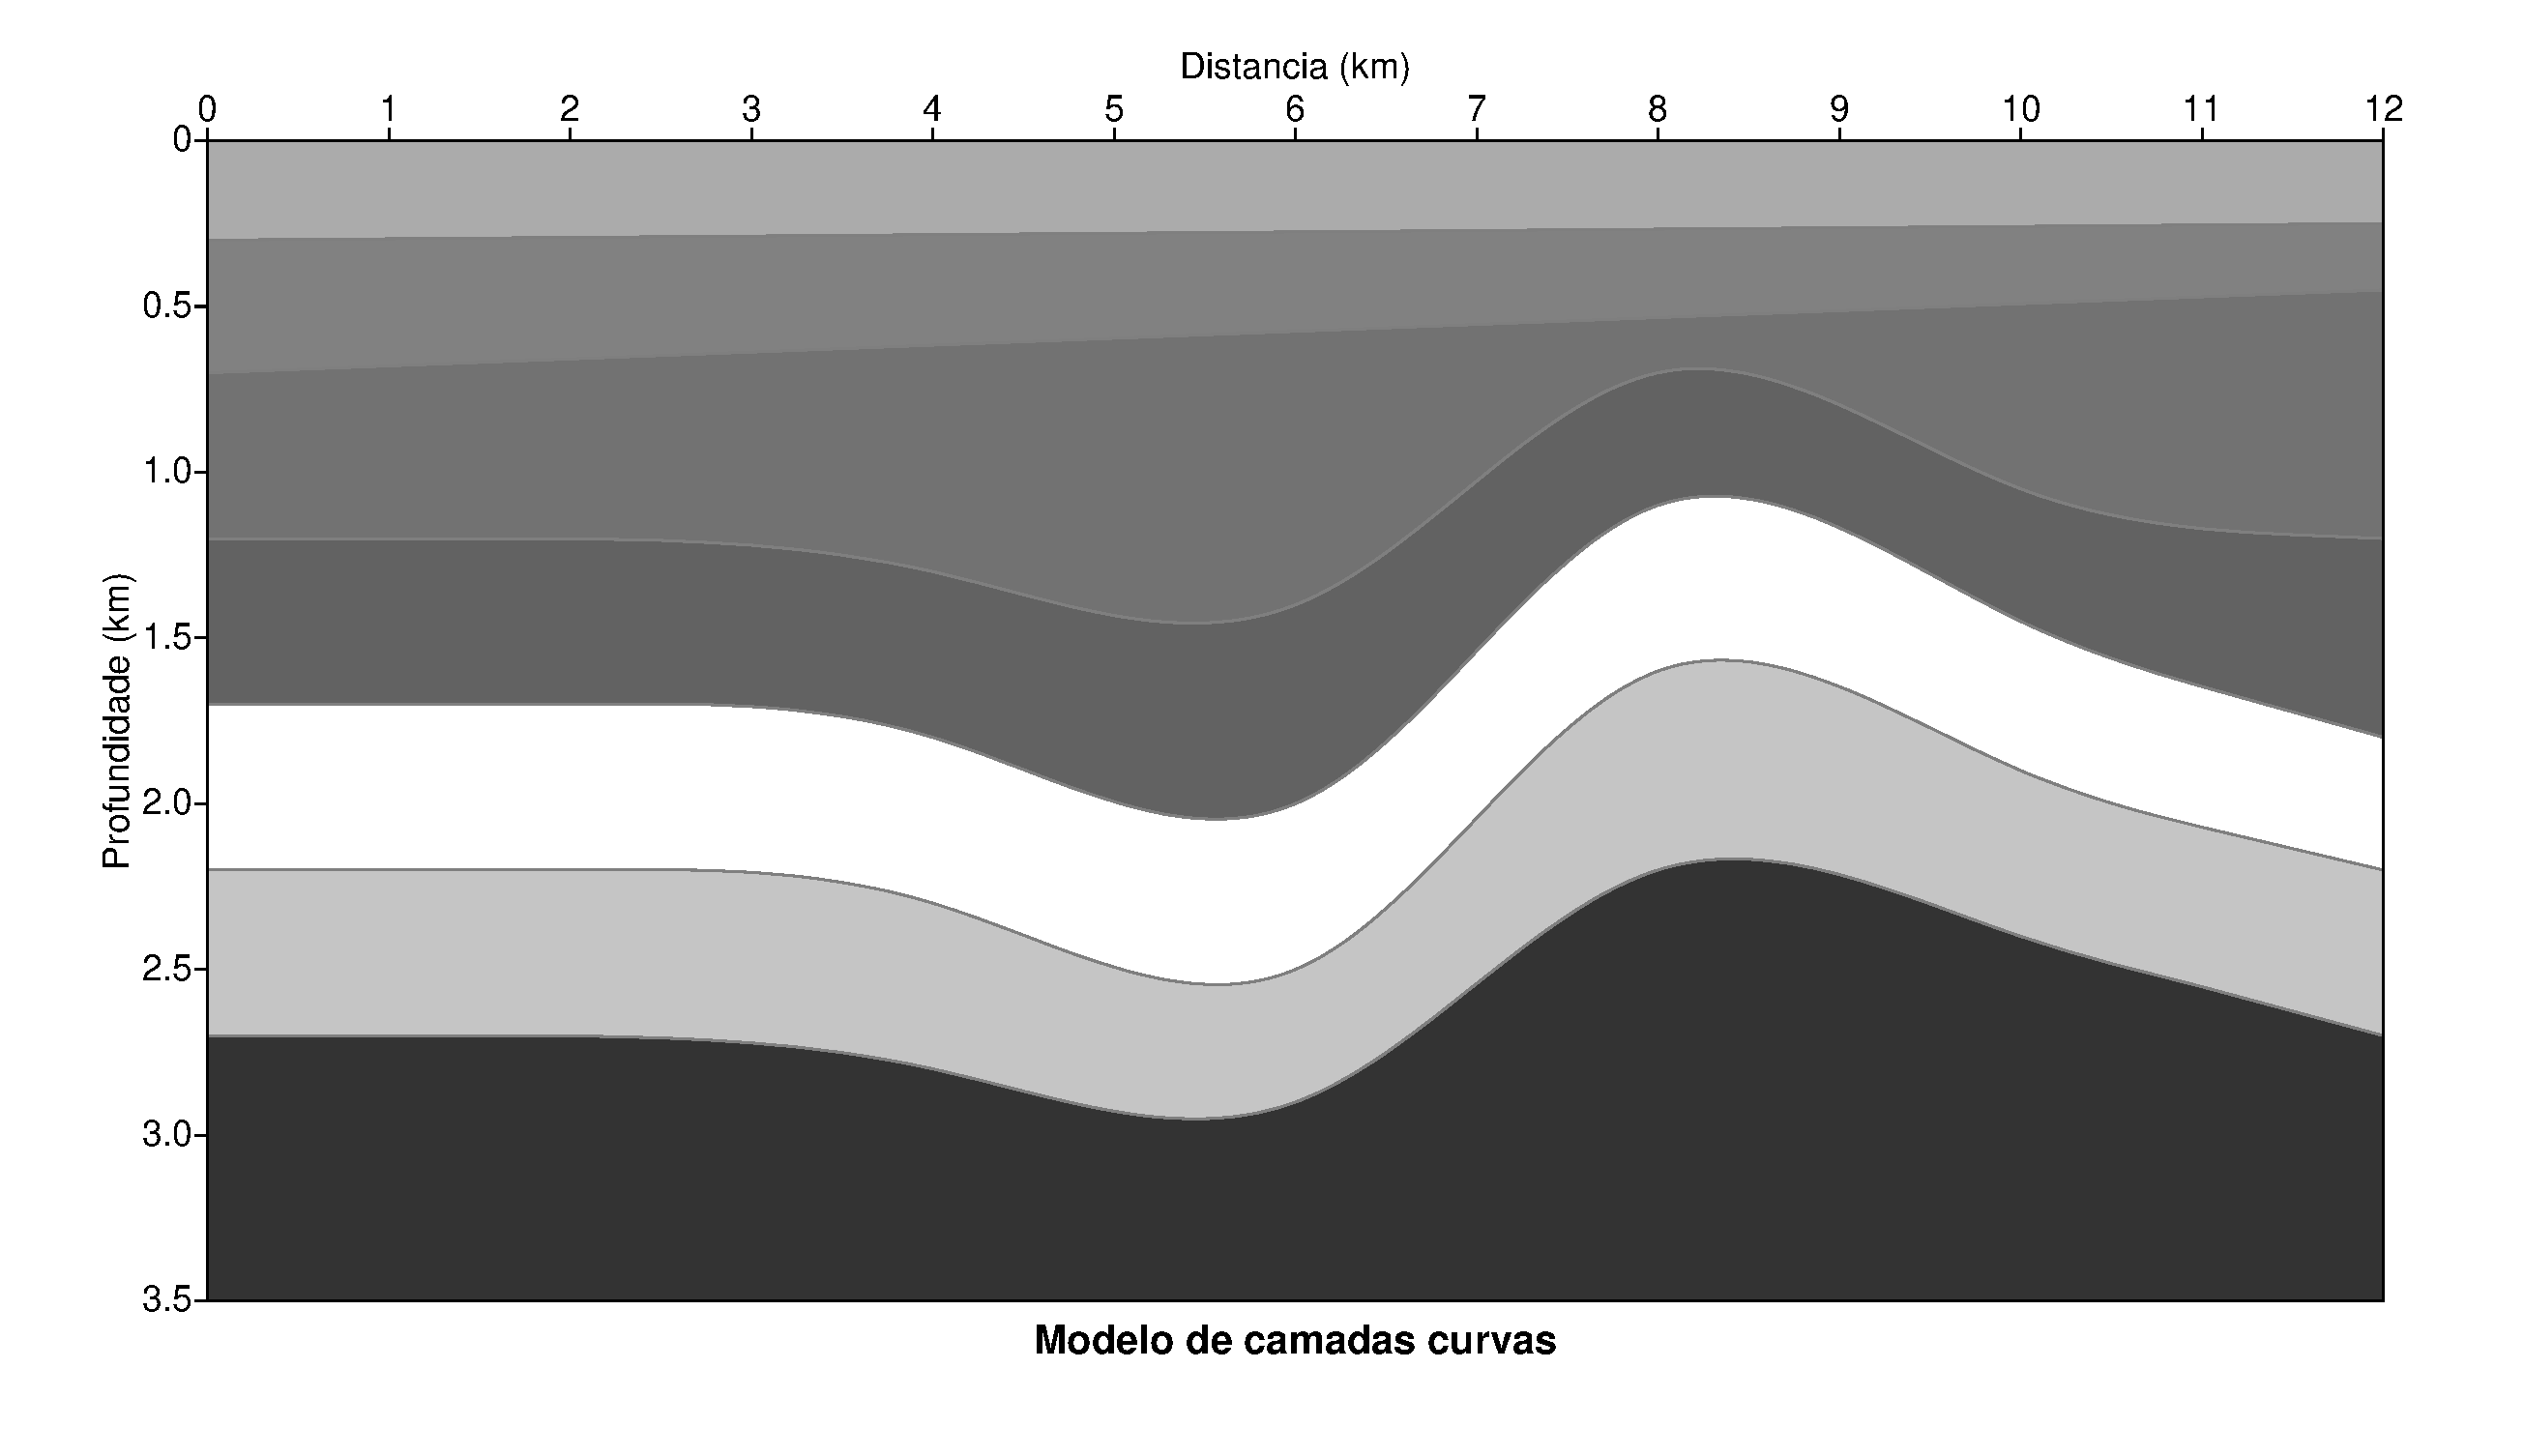
\includegraphics[totalheight=14cm]{figuras/cap2/vagarosidade.eps}
\caption{Modelo 2D de camadas curvas.}
\label{fig:vagarosidade}
\end{figure}
\end{landscape}

\begin{landscape}
\begin{figure}[H]
\centering
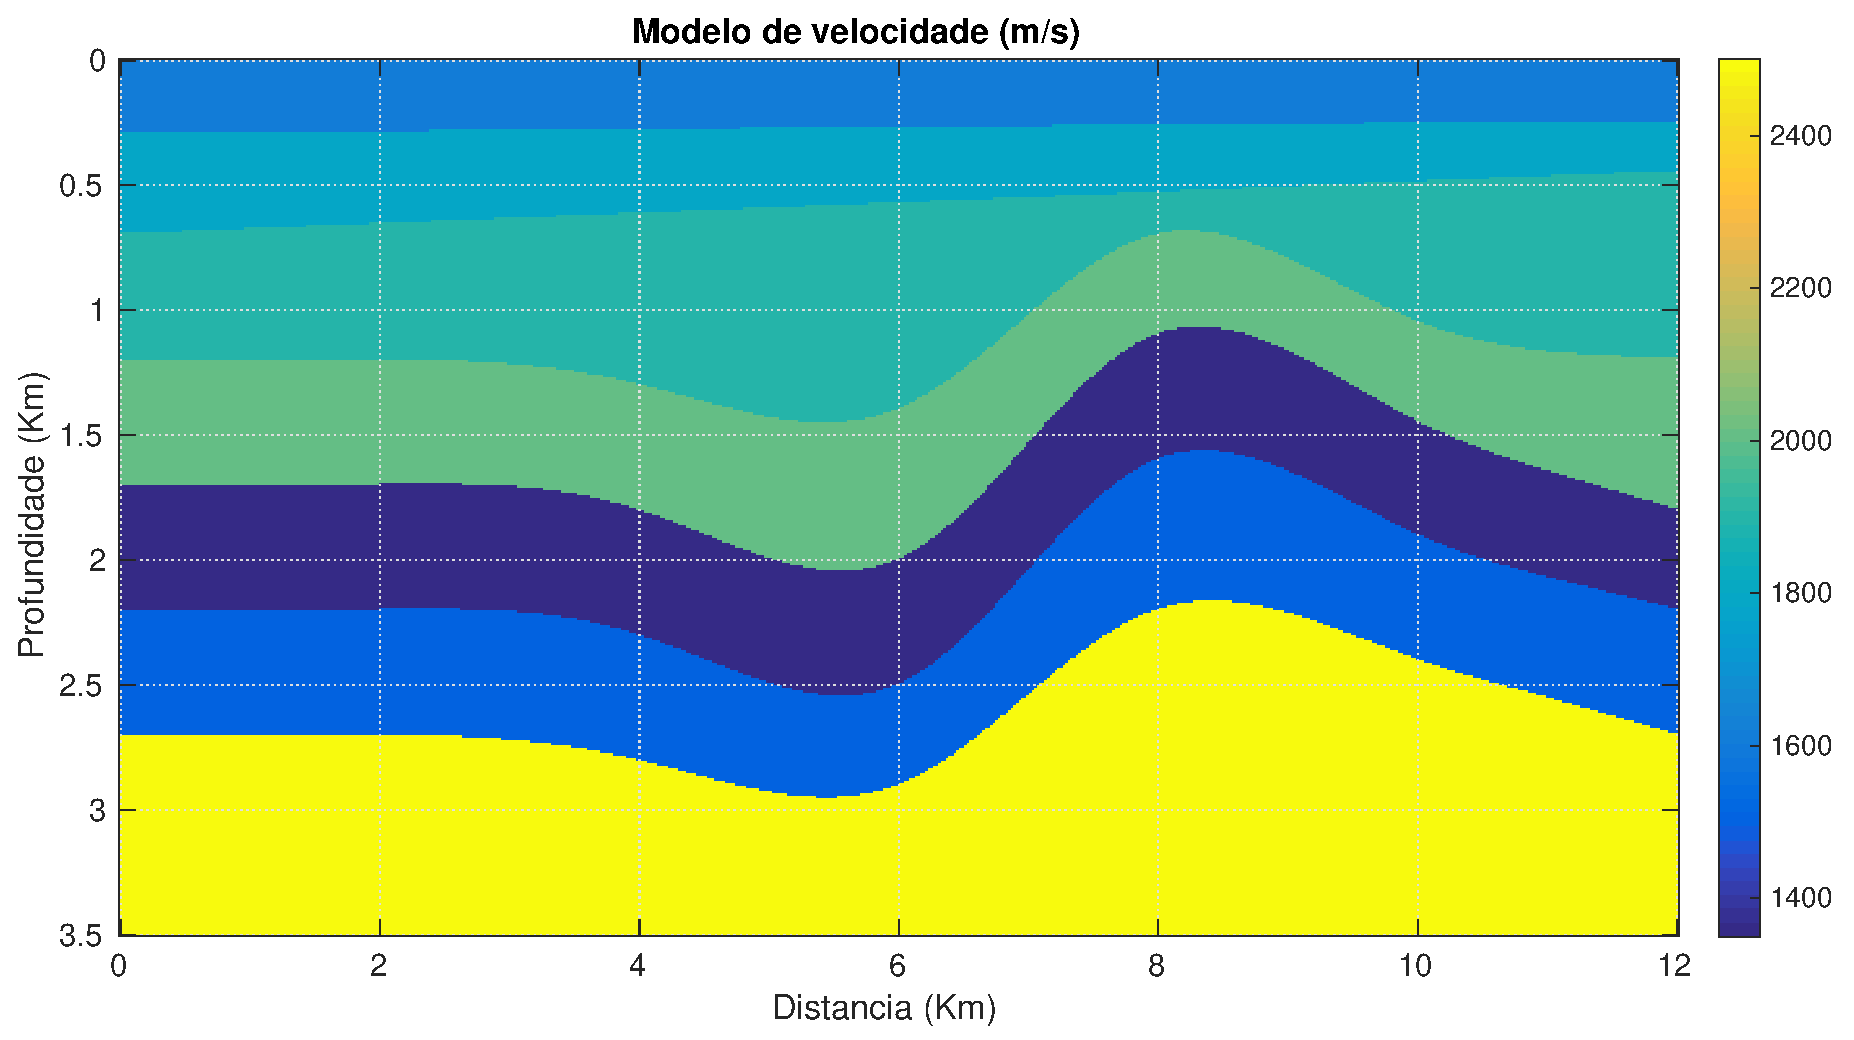
\includegraphics[totalheight=14cm]{figuras/cap2/modelo_de_velocidade.eps}
\caption{Modelo 2D de velocidade das camadas referente a figura (\ref{fig:vagarosidade}).}
\label{fig:modelo_velocidade}
\end{figure}
\end{landscape}

\section{PARÂMETROS DE AQUISIÇÃO}

Para se obter um sismograma sintético a partir de uma modelagem sísmica é preciso definir, inicialmente, a geometria de aquisição de dados. Neste sistema devem ser estabelecidas: a quantidade de receptores, a distância entre a fonte e o primeiro receptor e a distância entre os demais receptores.

Utilizamos a subrotina \textit{triseis} do \textit{Seismic Unix} (Anexo B) que tem por objetivo gerar os traços sísmicos referente a resposta do modelo de camadas curvas. A subrotina se basiea na teoria de raios e gera os sismogramas sintéticos de feixes Gaussianos, a partir de um modelo triangularizado preenchido (triângulos) com os valores de vagarosidade. Os parâmetros requeridos pela subrotina são:

\begin{itemize}
 \item xs: coordenadas da fonte
 \item zs: profundidade da fonte em superfície
 \item xg: coordenada dos receptores em superfície
 \item zg: profundidade dos receptores
\end{itemize}

A operação da subrotina funciona funciona dentro de três loops sucessivos. Isto ocorre de forma que o \textit{i-loop} referente às posições da fonte depende da conclusão do \textit{j-loop} que descreve cada posição de receptor, que por sua vez, depende de \textit{k-loop}, que mapeia cada refletor separadamente. Portanto, todos os raios referente ao primeiro refletor (localizados na interface 2), são armazenados nos receptores, para o primeiro tiro. Em seguida todos os raios varrem o segundo refletor (interface 3) e são armazenados em cada receptor novamente ainda para o primeiro tiro. Quando todos os refletores são mapeados é que ocorre o loop da posição da fonte varrendo a dimensão do modelo.

O arranjo utilizado ``split-spread'' simétrico figura (\ref{fig:split_spread}) possui o mesmo número de recpetores (geofones) equiespaçados linearmente em ambos os lados da coordenada de tiro. A distância entre a fonte e o primeiro receptor é conhecida como afastamento mínimo. A figura (\ref{fig:afastamento_min}) mostra o afastamento mínimo entre fonte e receptor.

\begin{figure}[H]
\centering
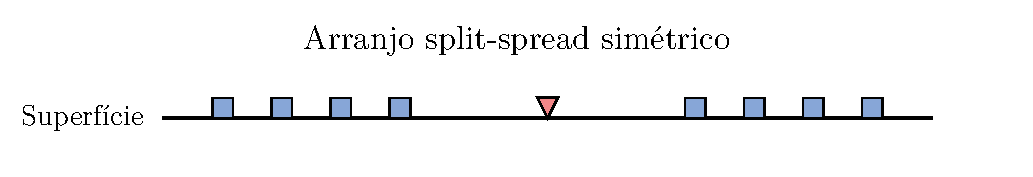
\includegraphics[height=2.5cm]{figuras/cap2/split_spread.pdf}
\caption{Arranjo split spread simétrico em relação a posição da fonte. Em vermelho a representação da fonte e em azul os recpetores (geofones).}
\label{fig:split_spread}
\end{figure}

\begin{landscape}
\begin{figure}[H]
\centering
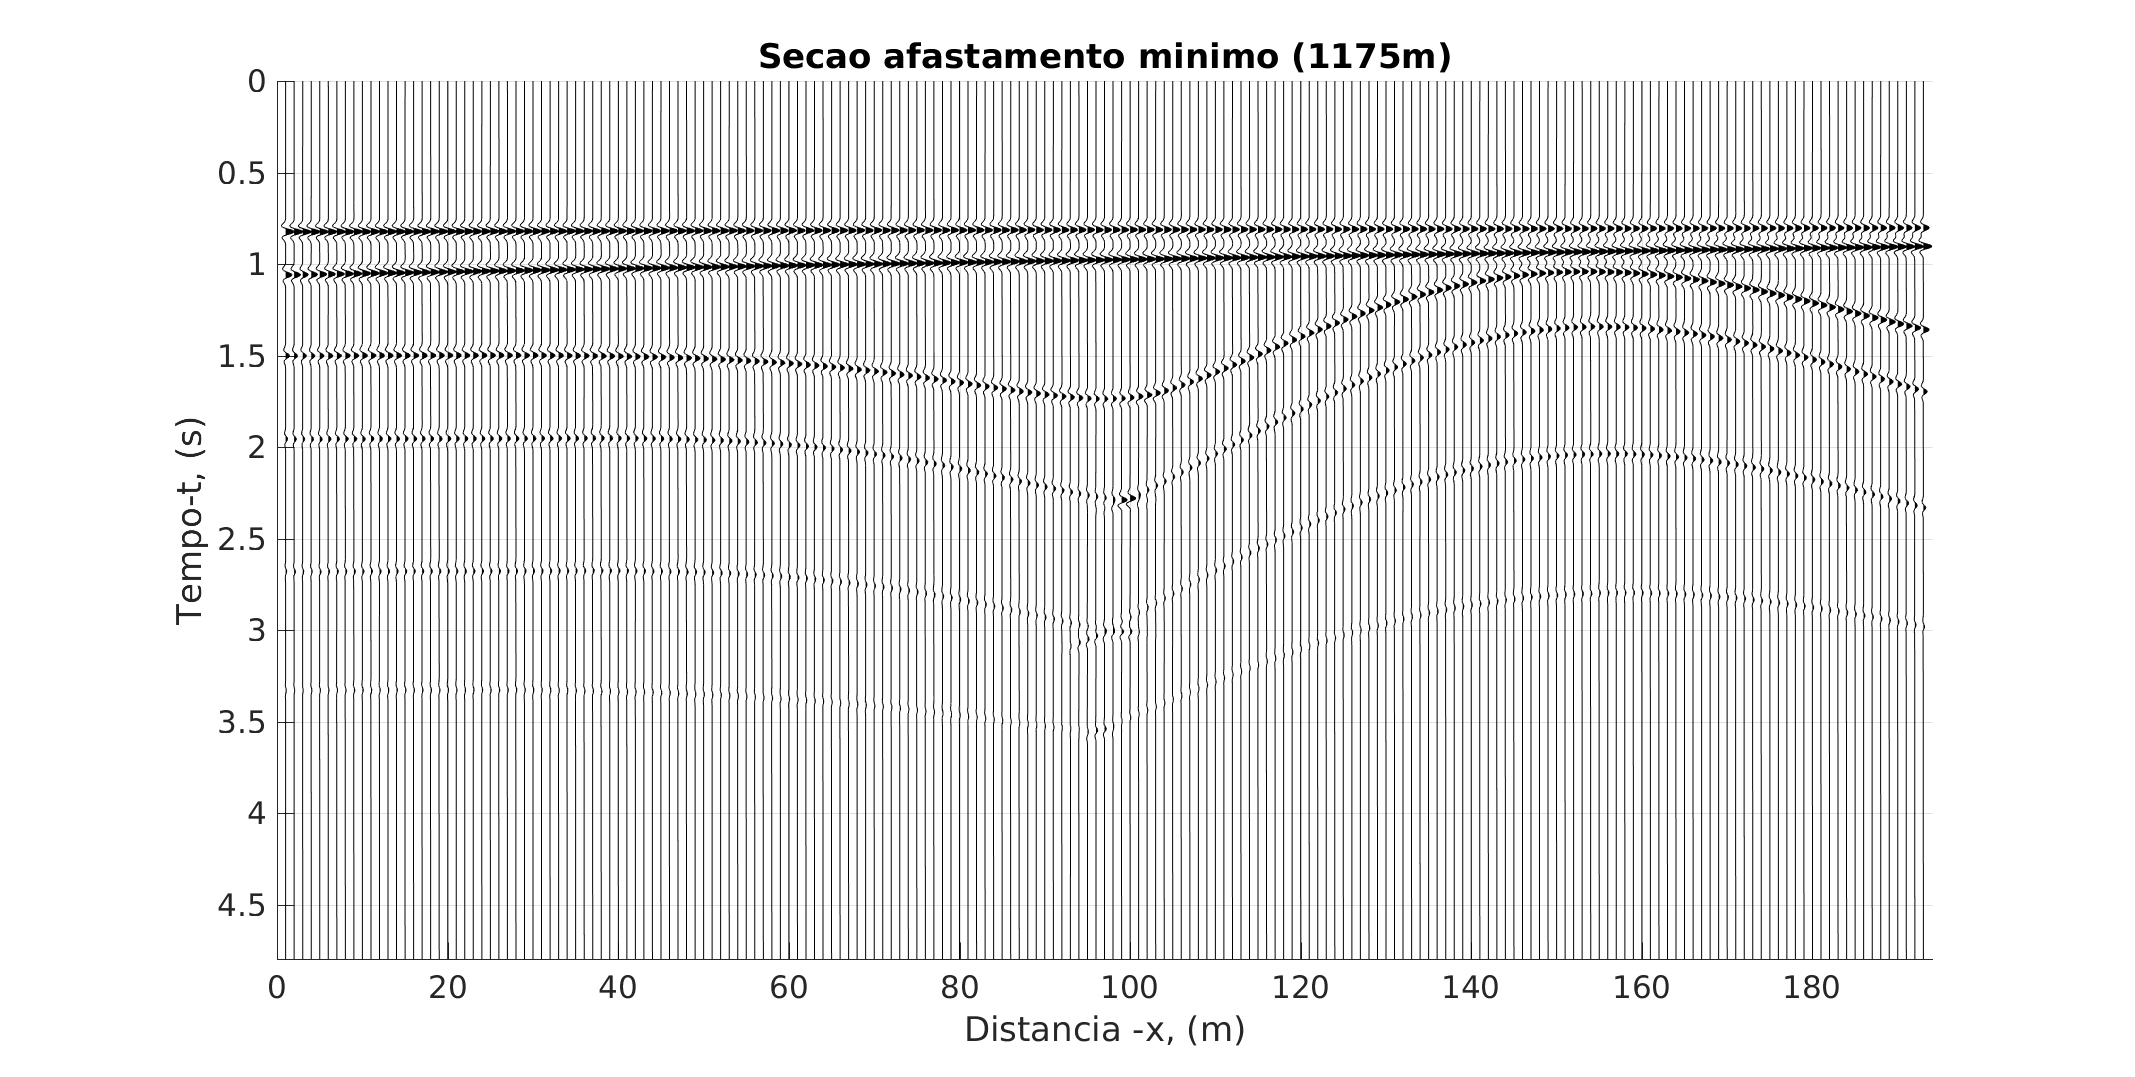
\includegraphics[totalheight=14cm]{figuras/cap2/wigb_plot.pdf}
\caption{Afastamento mínimo entre fonte e receptor.}
\label{fig:afastamento_min}
\end{figure}
\end{landscape}
